
%! program = pdflatex

\documentclass[12pt]{article}
\usepackage{amsmath}
\usepackage{natbib}
\usepackage{graphicx}
\usepackage{amssymb}
\usepackage{epstopdf}
\usepackage{float} % to keep the figures in place

\usepackage{color}
\newcommand{\cred}{ \color{red}}
\newcommand{\cgreen}{\color{green}}
\newcommand{\cblue}{\color{blue}}
\newcommand{\cmag}{\color{magenta}}
\newcommand{\bn}{\begin{enumerate}}
\newcommand{\en}{\end{enumerate}}
\newcommand{\bi}{\begin{itemize}}
\newcommand{\ei}{\end{itemize}}
\newcommand{\be}{\begin{eqnarray}}
\newcommand{\ee}{\end{eqnarray}}
\newcommand{\by}{\begin{eqnarray*}}
\newcommand{\ey}{\end{eqnarray*}}
\renewcommand{\labelenumi}{(\alph{enumi}) }
%
\usepackage[margin=2.2cm, includehead]{geometry}% see geometry.pdf on how to lay out the page. There's lots.
\geometry{letterpaper} % or letter or a5paper or ... etc
% \geometry{landscape} % rotated page geometry
%\bibpunct{(}{)}{;}{a}{,}{,}
%\setlength{\textwidth}{16cm}
%\setlength{\textheight}{21cm}
\def\nonumber{\global\@eqnswfalse}
\newcounter{parnum}
\newcommand{\N}{%
  \noindent\refstepcounter{parnum}%
   \makebox[\parindent][l]{\textbf{[\arabic{parnum}]}}\quad  }
% Use a generous paragraph indent so numbers can be fit inside the
% indentation space.
\setlength{\parindent}{1.5em}

% See the ``Article customise'' template for come common customisations

\date{}
%\date{} % delete this line to display the current date

%%% BEGIN DOCUMENT
\usepackage{Sweave}
\begin{document}
\Sconcordance{concordance:HW4.tex:HW4.Rnw:%
1 47 1 1 0 22 1 1 38 4 0 1 2 20 1 1 3 19 0 1 1 3 0 1 2 1 0 1 2 1 1 1 2 %
5 0 1 2 3 1 1 3 4 0 1 2 1 1 1 7 4 0 1 2 5 1 1 2 5 0 1 2 14 1 1 3 6 0 1 %
4 18 0 1 1 3 0 2 2 1 0 1 1 4 0 1 2 3 1 1 3 4 0 1 2 1 7 4 0 1 2 3 1 1 3 %
1 2 5 1 1 2 1 0 1 1 4 0 1 2 11 1 1 3 23 0 2 2 4 0 1 2 3 1 1 13 1 2 2 1 %
1 3 4 0 1 2 3 1 1 4 1 2 3 1 1 4 1 2 5 1 1 2 1 0 1 1 4 0 1 2 10 1 1 7 9 %
0 1 2 1 1}

%\large
%\maketitle
\newtheorem{thm}{Theorem}[section]
\newtheorem{cor}[thm]{Corollary}
\newtheorem{lem}[thm]{Lemma}
\newtheorem{prop}[thm]{Proposition}
\newtheorem{defn}[thm]{Definition}
\newtheorem{exam}[thm]{Example}
\newtheorem{qstn}[thm]{Question}

%%%
\newpage
\begin{center}
{\bf Homework 4 - STAT 511}\\
Amal Agarwal
\end{center}
%==========================
\section*{Answer 3}
\bn
\item
It is given that $MSD(t)=E[X^2(t)]$. From the given data, it can be observed that the position of different particles have been given for 4 time points viz. 5, 10, 15, 20. Thus for each time point, we can estimate the MSD (mean of the squared distances) by approximating it with the sample mean of the squared distances at each of the time points. 
\begin{Schunk}
\begin{Soutput}
[1]  574.3304 1272.7540 1755.0098 2327.1401
\end{Soutput}
\end{Schunk}
\item Now MSD scales according to the following power law:
\begin{equation*}
\begin{aligned}
MSD(t)=\gamma t^{\alpha}
\end{aligned}
\end{equation*}
Taking log of the above equation, we get
\begin{equation*}
\begin{aligned}
log(MSD(t))= log(\gamma) + \alpha log(t)
\end{aligned}
\end{equation*}
Now since we know the estimated MSD at each of the time points from the above data, we can fit the following model
\begin{equation*}
\begin{aligned}
log(\widehat{MSD}_{i}(t_{i}))= \beta_0 + \alpha log(t_{i}) + \epsilon_{i}, \hspace{0.1in} \epsilon_{i} \sim N(0,\sigma^2)
\end{aligned}
\end{equation*}
The summary of the model fit and the plot of $log(\widehat{MSD})$ vs. $log(t)$ with the fitted line are given as follows

\begin{figure}[H]
\begin{Schunk}
\begin{Soutput}
Call:
lm(formula = I(log(xsq.mean)) ~ I(log(tm)))

Residuals:
       1        2        3        4 
-0.03140  0.06938 -0.01586 -0.02212 

Coefficients:
            Estimate Std. Error t value Pr(>|t|)    
(Intercept)  4.77096    0.13508   35.32 0.000801 ***
I(log(tm))   1.00261    0.05492   18.26 0.002987 ** 
---
Signif. codes:  0 ‘***’ 0.001 ‘**’ 0.01 ‘*’ 0.05 ‘.’ 0.1 ‘ ’ 1 

Residual standard error: 0.05718 on 2 degrees of freedom
Multiple R-squared: 0.994,	Adjusted R-squared: 0.9911 
F-statistic: 333.3 on 1 and 2 DF,  p-value: 0.002987 
\end{Soutput}
\begin{Soutput}
(Intercept)  I(log(tm)) 
   4.770961    1.002612 
\end{Soutput}
\end{Schunk}
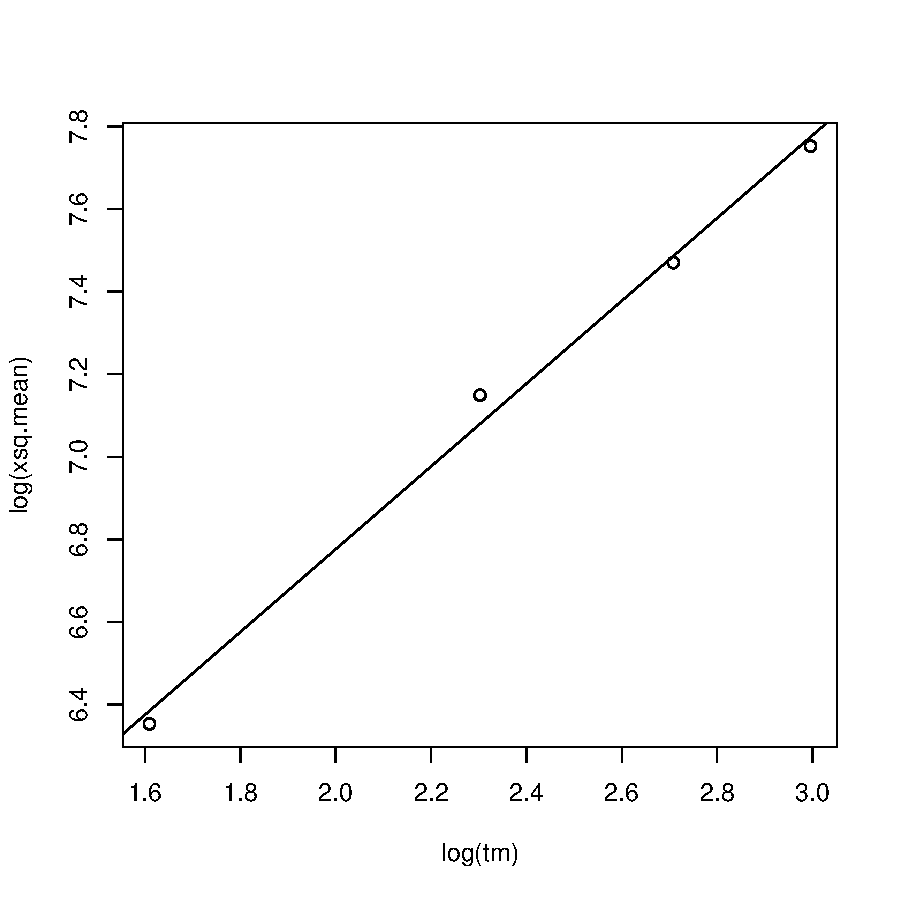
\includegraphics{HW4-002}
\end{figure}
\item Clearly the estimated value of $\alpha$ is 
\begin{Schunk}
\begin{Soutput}
I(log(tm)) 
  1.002612 
\end{Soutput}
\end{Schunk}
It is not needed to estimate $\gamma$ here. However, even if it was needed we could not have done it since $\widehat{log(\gamma)} \neq log(\hat{\gamma})$. This can be verified by Jensen's inequality which gives $E(\widehat{log(\gamma)}) \geq log(E(\hat{\gamma}))$.
\item The assumptions of the model can verified as follows:
\begin{itemize}
\item The mean of the residuals can be calculated as
\begin{Schunk}
\begin{Soutput}
[1] -1.734723e-18
\end{Soutput}
\end{Schunk}
which is very close to zero thus verifying our assumption of $E(\epsilon)=0$
\item The column rank of the design matrix X can be calculated as:
\begin{Schunk}
\begin{Soutput}
[1] 2
\end{Soutput}
\end{Schunk}
which confirms our assumption of full column rank design matrix.
\item To check for homoscedasticity, the plot of residuals against the predictor doesn't help much here since we only have 4 points. Similarily the QQ plot of residuals which is the diagnostic for normality also fails.
\clearpage

\item Plot of $x^2$ vs. t
\begin{figure}[H]
\begin{Schunk}
\begin{Sinput}
> plot(t,x^2)
\end{Sinput}
\end{Schunk}
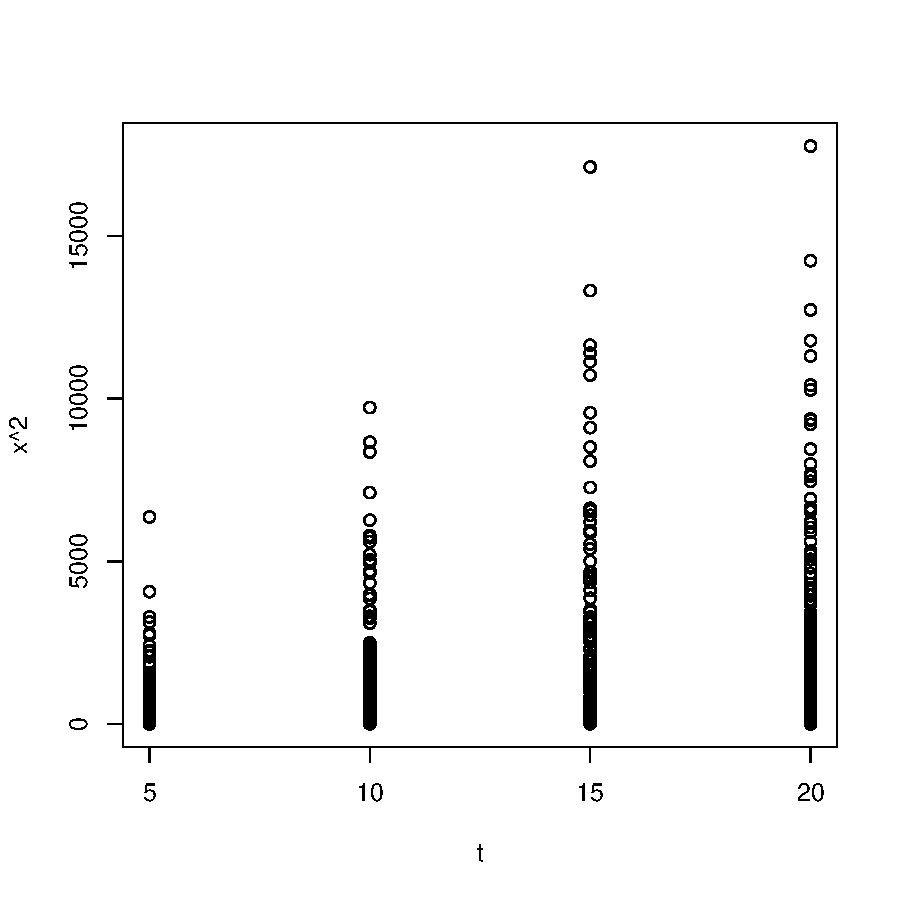
\includegraphics{HW4-006}
\end{figure}
The above plot shows a heteroscedastic behaviour of $x^2$ with t. Further tha variance increases as t is increased and thus the errors are correlated.
\item We can't comment much on normality assumption in our model but still we can say that individually the mean of $x^2$ at different time points must follow a normal distribution (since $n=200>>30$ for each $t_i$) by central limit theorem.
\end{itemize}
\en
\clearpage

\section*{Answer 4}
\bn
\item The following model was fitted to the given data:
\begin{equation*}
\begin{aligned}
goldtime_i=\beta_0+\beta_1 year_i +\epsilon_i, \hspace{0.1in} \epsilon_i \sim N(0,\sigma^2)
\end{aligned}
\end{equation*}
\begin{Schunk}
\begin{Soutput}
'data.frame':	42 obs. of  3 variables:
 $ year    : int  1900 1904 1908 1912 1920 1924 1928 1932 1936 1948 ...
 $ goldtime: num  11 11 10.8 10.8 10.8 10.6 10.8 10.3 10.3 10.3 ...
 $ gender  : Factor w/ 2 levels "M","W": 1 1 1 1 1 1 1 1 1 1 ...
\end{Soutput}
\begin{Soutput}
Call:
lm(formula = oly$goldtime ~ oly$year)

Residuals:
    Min      1Q  Median      3Q     Max 
-0.6976 -0.5089 -0.2196  0.4869  1.2269 

Coefficients:
             Estimate Std. Error t value Pr(>|t|)    
(Intercept) 26.663985   5.865382   4.546 4.97e-05 ***
oly$year    -0.008138   0.002991  -2.721   0.0096 ** 
---
Signif. codes:  0 ‘***’ 0.001 ‘**’ 0.01 ‘*’ 0.05 ‘.’ 0.1 ‘ ’ 1 

Residual standard error: 0.5679 on 40 degrees of freedom
Multiple R-squared: 0.1561,	Adjusted R-squared: 0.135 
F-statistic: 7.401 on 1 and 40 DF,  p-value: 0.0096 
\end{Soutput}
\begin{Soutput}
[1] 0.5678969
\end{Soutput}
\end{Schunk}
\begin{figure}[H]
\begin{Schunk}
\begin{Sinput}
> plot(year,goldtime)
> abline(fit)
\end{Sinput}
\end{Schunk}
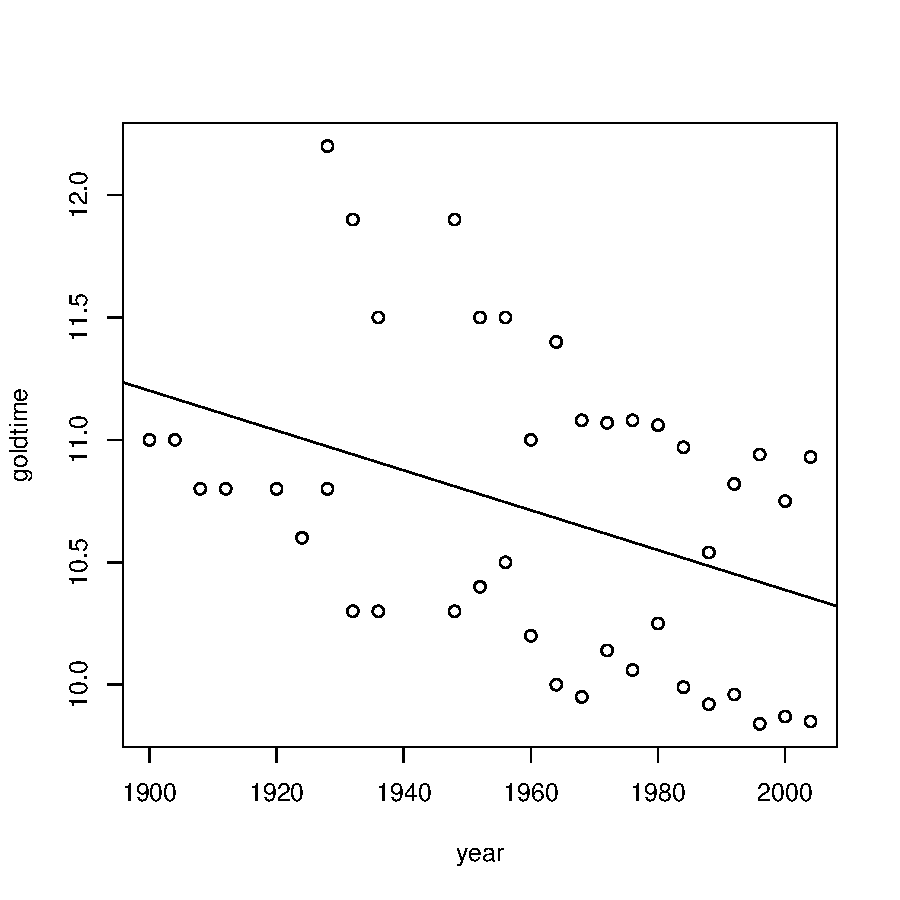
\includegraphics{HW4-008}
\end{figure}
Clearly there is a set of points above fitted line and there is another set below it which shows that we are missing the effect of a categorical covariate.\\
Diagnostics:\\
The mean of the residuals can be calculated as 
\begin{Schunk}
\begin{Soutput}
[1] 3.003498e-18
\end{Soutput}
\end{Schunk}
which is very close to zero thus verifying our assumption of $E(\epsilon)=0$. The column rank of the design matrix X can be calculated as:
\begin{Schunk}
\begin{Soutput}
[1] 2
\end{Soutput}
\end{Schunk}
which confirms our assumption of full column rank design matrix.
\clearpage
The residual plot of the corresponding fit is given as follows:
\begin{figure}[H]
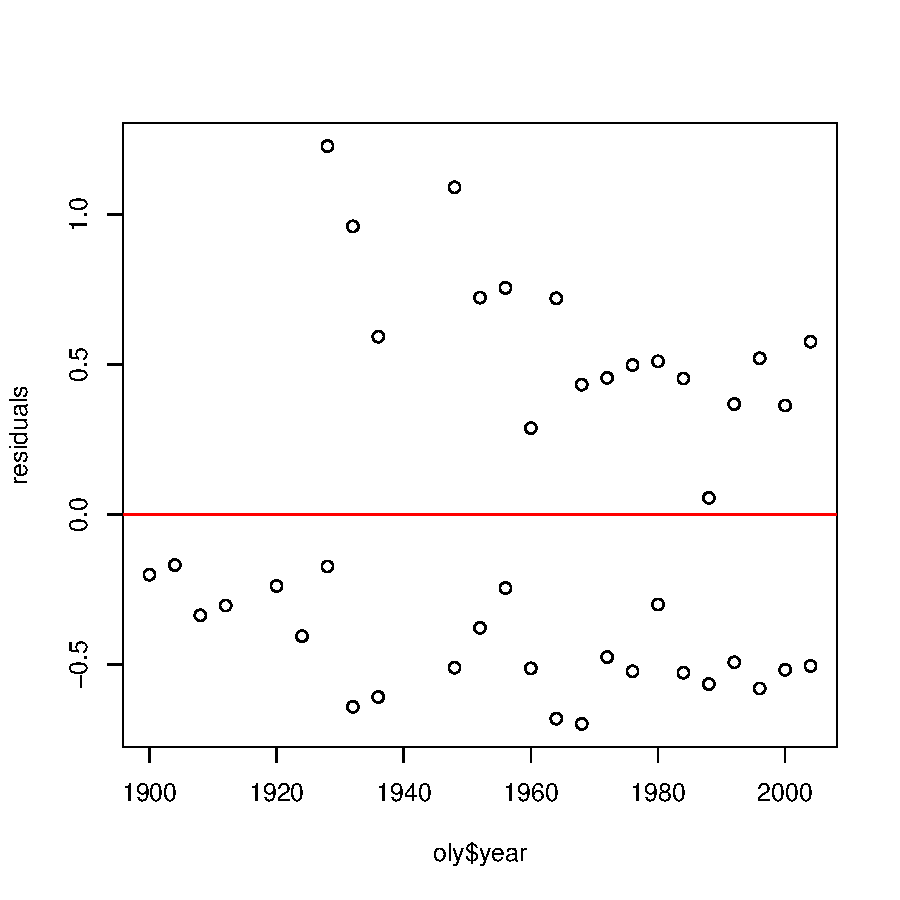
\includegraphics{HW4-011}
\end{figure}
This residuals are not uniformly distributed around zero which shows that our assumption of homoscedascity is not satisfied here.

\clearpage
To check for our normality assumption, QQ plot of the residuals is given as follows:
\begin{figure}[H]
\begin{Schunk}
\begin{Sinput}
> qqnorm(residuals)
> qqline(residuals)
\end{Sinput}
\end{Schunk}
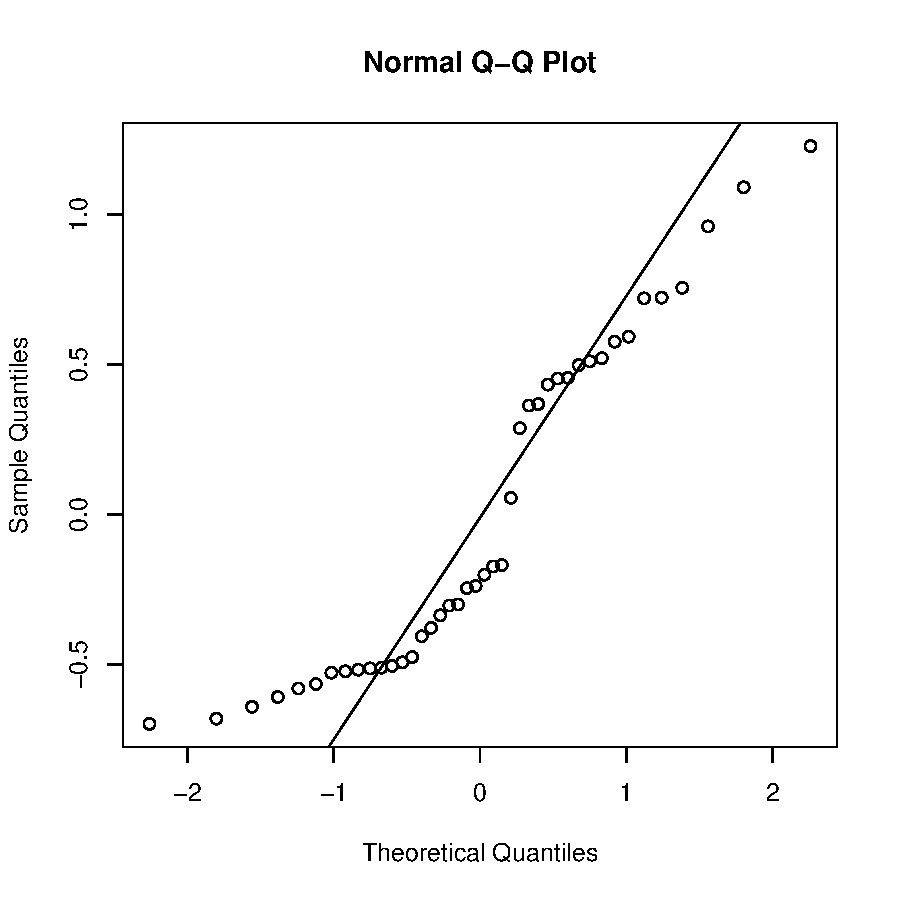
\includegraphics{HW4-012}
\end{figure}
Although the short tails on both the left and right sides don't matter much, still this is not very close to normality.
Interpretation of the effect of year on gold medal time in 100 m race: Estimated value of the $\beta_1$, i.e. $\hat{\beta_1}$ shows the mean decrease of $-0.008 s$ in goldtime per unit increase in year. Note that the effect of gender has not been taken into account in this model.

\item Considering the transformations and interactions, the final model that I think is most appropriate for the given data is:
\begin{equation*}
\begin{aligned}
goldtime_i=\beta_0 + \beta_1 \left(\dfrac{1}{year_i}\right) + \beta_2 (gender_i) + \beta_3 (year_i*gender_i) + \epsilon_i, \hspace{0.1in} \epsilon_i \sim N(0,\sigma^2)
\end{aligned}
\end{equation*}

The summary of the fit including the estimated parameters are given as follows:
\begin{Schunk}
\begin{Soutput}
Call:
lm(formula = goldtime ~ I(1/year) + gender + (year:gender), data = oly)

Residuals:
     Min       1Q   Median       3Q      Max 
-0.36163 -0.06361  0.00333  0.08119  0.33698 

Coefficients:
               Estimate Std. Error t value Pr(>|t|)    
(Intercept)  -5.295e+02  2.600e+02  -2.036 0.048931 *  
I(1/year)     5.476e+05  2.537e+05   2.159 0.037430 *  
genderW       1.671e+01  4.350e+00   3.841 0.000464 ***
genderM:year  1.328e-01  6.663e-02   1.993 0.053646 .  
genderW:year  1.249e-01  6.566e-02   1.902 0.065007 .  
---
Signif. codes:  0 ‘***’ 0.001 ‘**’ 0.01 ‘*’ 0.05 ‘.’ 0.1 ‘ ’ 1 

Residual standard error: 0.1631 on 37 degrees of freedom
Multiple R-squared: 0.9356,	Adjusted R-squared: 0.9287 
F-statistic: 134.5 on 4 and 37 DF,  p-value: < 2.2e-16 
\end{Soutput}
\end{Schunk}
The estimated variance is
\begin{Schunk}
\begin{Soutput}
[1] 0.1630664
\end{Soutput}
\end{Schunk}

\clearpage
The fitted model is given as:
\begin{figure}[H]
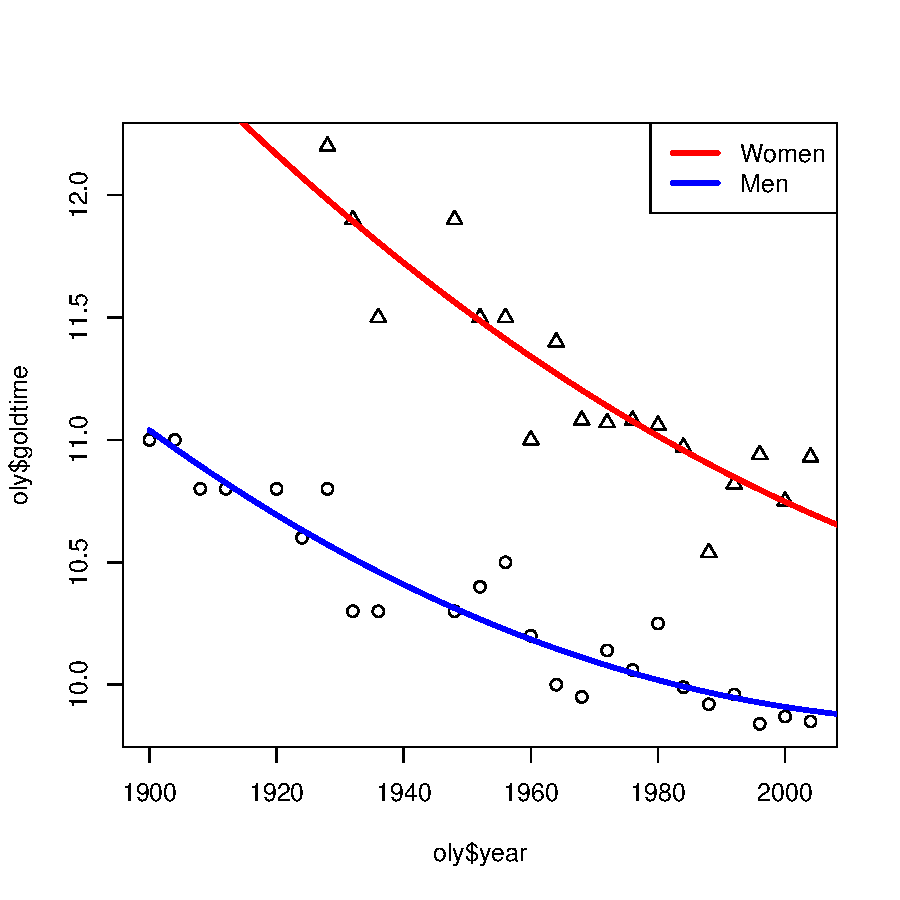
\includegraphics{HW4-015}
\end{figure}
Diagnostics:\\
The mean of the residuals can be calculated as 
\begin{Schunk}
\begin{Soutput}
[1] -4.252912e-18
\end{Soutput}
\end{Schunk}
which is very close to zero thus verifying our assumption of $E(\epsilon)=0$.
\clearpage
The residual plots of the corresponding fit is given as follows:
\begin{figure}[H]
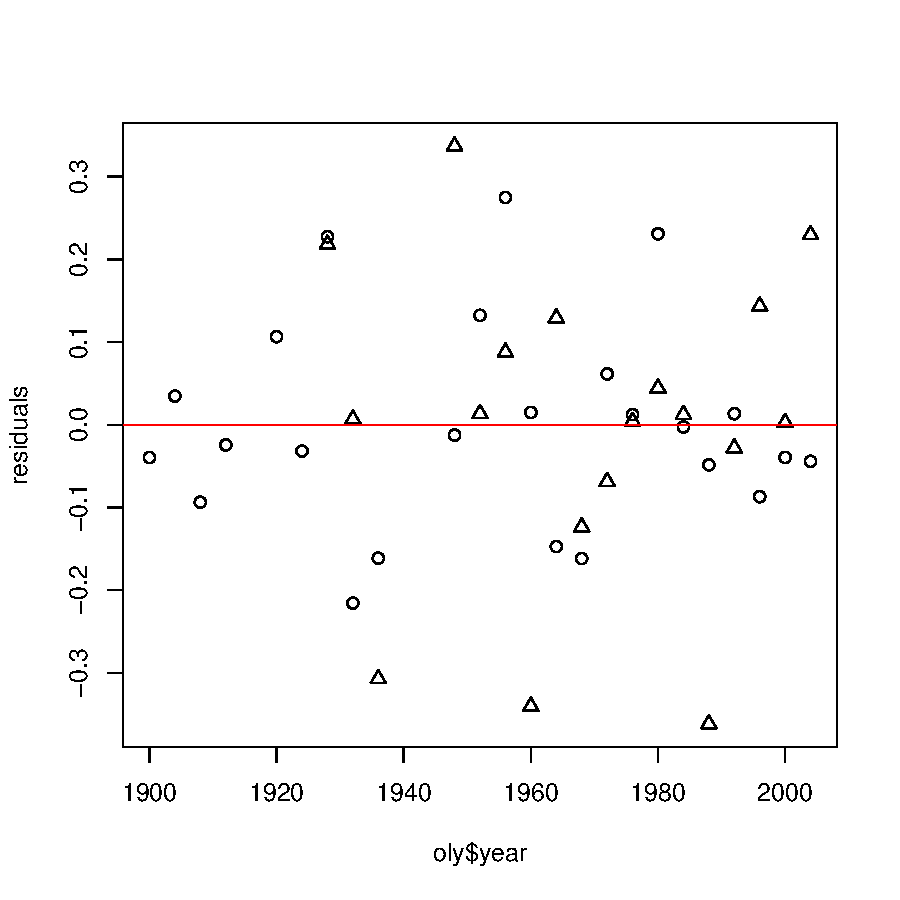
\includegraphics{HW4-017}
\end{figure}
This shows that the residuals are uniformly distributed with respect to year and hence uncorrelated. Thus our assmption of independent errors is satisfied.

\begin{figure}[H]
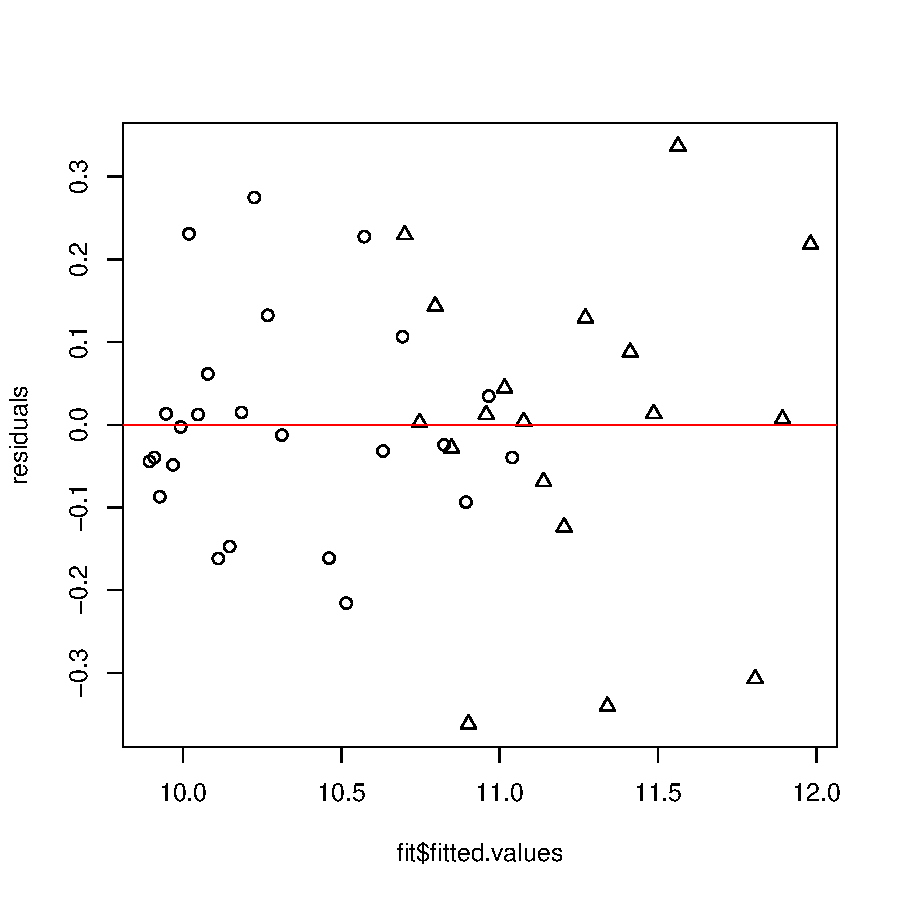
\includegraphics{HW4-018}
\end{figure}
This shows that the residuals are uniformly distributed with respect to fitted values and hence our assmption of homoscedascity is satisfied.

\clearpage
To check for our normality assumption, QQ plot of the residuals is given as follows:
\begin{figure}[H]
\begin{Schunk}
\begin{Sinput}
> qqnorm(residuals)
> qqline(residuals)
\end{Sinput}
\end{Schunk}
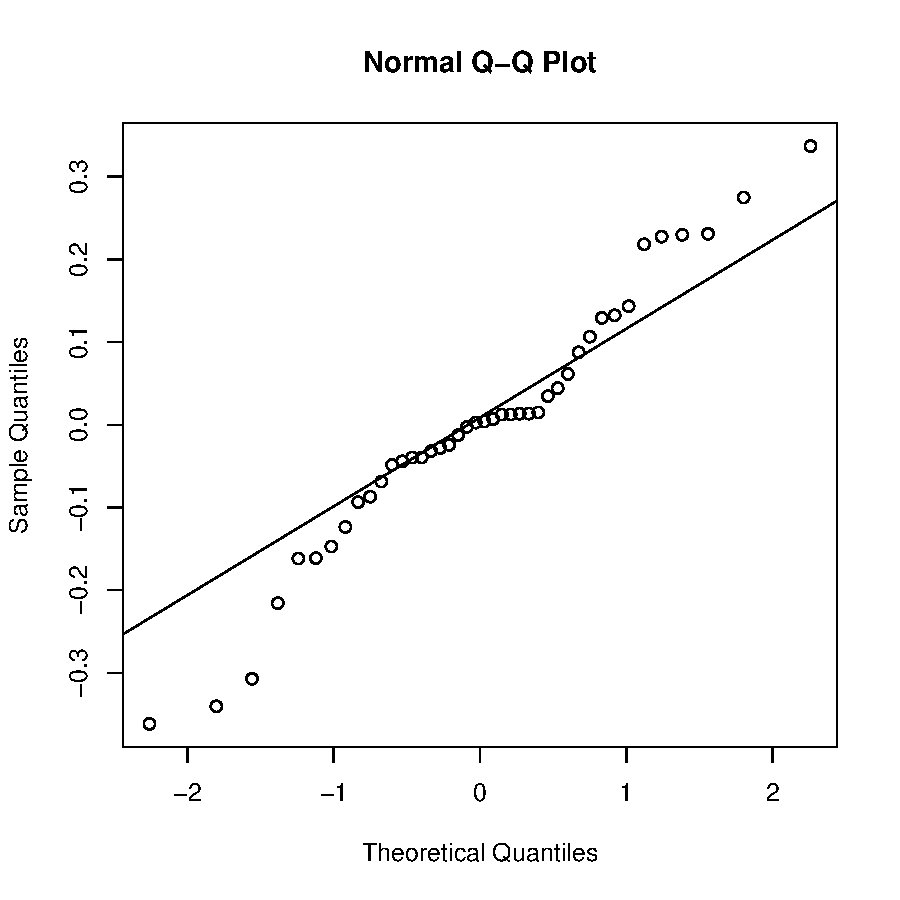
\includegraphics{HW4-019}
\end{figure}
The fat tails on both the ends clearly shows significant deviation from normality.

Note that this model seemed to be best since both our assumptions of homoscedascity and independent errors are best verified in this case. However our assumption of normality does not hold good, which is fine since it is not that important.

It is not possible to construct partial residual plots and check the assumption of linearity since we have an interaction term.

Interpretation of the effect of predictor variables on gold medal time in 100 m race: Estimated value of the $\beta_1$, i.e. $\hat{\beta_1}= 5.476 \times 10^5$ shows that the mean gold medal time decreases with increase in year for both Men's and Women's races. $\hat{\beta_2}= 16.71$ shows that the mean gold medal time is higher for Women than Men. Further $\hat{\beta_3}$ is 0.1328 for Men and 0.1249 for Women which shows that the mean gold time decreases at a faster rate with respect to year for women than men.

\item The predicted gold medal time values for Mens and Womens 100 m races in 1944 are 
respectively given as 10.32404 s and 11.58253 s. The corresponding R code is given as follows
\begin{Schunk}
\begin{Sinput}
> for (i in 1:length(x.vals)) {
+   if (x.vals[i]==1944) {
+     Women.1944.predicted<-f.vals.0[i]
+     Men.1944.predicted<-f.vals.1[i]
+   }
+ }
\end{Sinput}
\end{Schunk}
\en
\end{document}
